% __Markdown to \LaTeX __
% 金子達哉 \texttt{(id:catatsuy)}
% 

## 自己紹介

* 金子達哉
* はてな ID: catatsuy
* twitter: catatsuy

\begin{picture}(0,0)(0,0)
  \put(200,0){
\includegraphics[clip, height=35truemm]{catatsuy}}
\end{picture}

\vspace{-20pt}

URL:

* \url{http://www.catatsuy.org}
* \url{http://blog.catatsuy.org}
* \url{https://matw.co}

## 所属

* 東京工業大学(≠電通大)
* 情報工学科 4 年(9 月卒業予定)
* 吉瀬研究室
    * コンピュータアーキテクチャ
\if0
    * `C++` でハードウェアのシミュレーションをする DSL を提供するライブラリを高速化する研究をしています(詳しくは略)
\fi

## 就職活動

* はてなインターン 2012
* pixiv インターン

\vspace{-20pt}

\begin{center}
 \begin{tabular}{cc}
   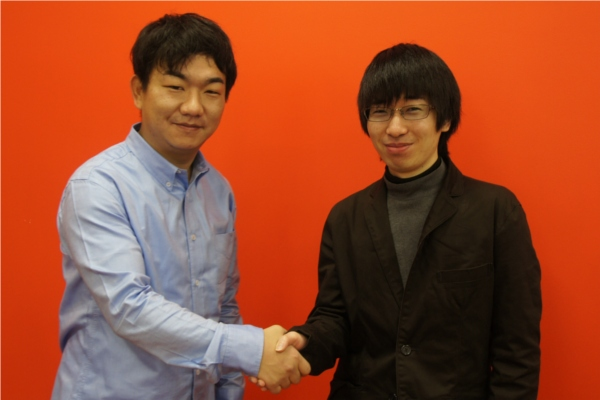
\includegraphics[clip, height=38truemm]{pixiv} & 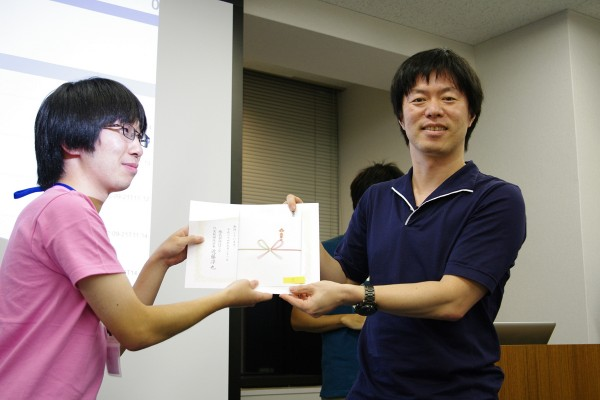
\includegraphics[clip, height=38truemm]{hatena} \\ 
  \end{tabular}
 \end{center}

## 

\begin{center}
 \LARGE
 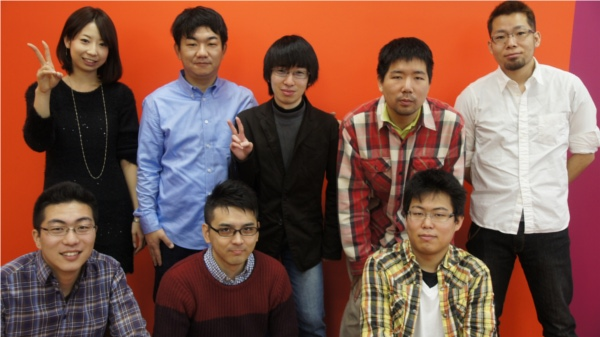
\includegraphics[clip, height=58truemm]{pixivall}\\
 \bfseries\gtfamily 10 月から 
\includegraphics[clip,
 height=25pt]{pixiv_logo} \hspace{2pt}  へ!
\end{center}


## 前回の Dentoo.LT

\vspace{-70pt}

`Acme::MorningMusume` の話をしました  
\url{http://blog.catatsuy.org/a/256}

\begin{picture}(0,0)(0,0)
 \put(100,-130){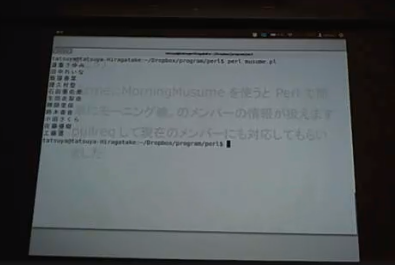
\includegraphics[clip, height=50truemm]{ustacme.png}}
\end{picture}

## 

\begin{center}
 \LARGE
 卒業したい
\end{center}

## 

\begin{center}
 \LARGE
 卒業論文\\
 (8 月提出のため)\\
 絶賛追い込みなう☆
\end{center}

## 突然の死刑宣告

\begin{picture}(0,0)(0,0)
 \put(30,-70){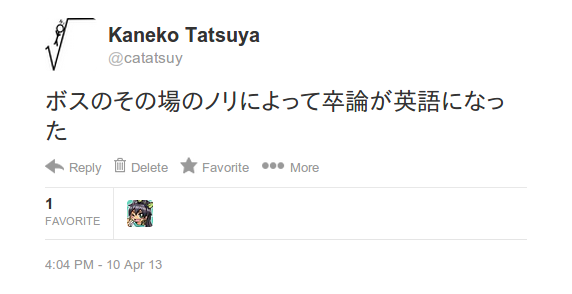
\includegraphics[clip, width=100truemm]{tweet.png}}
\end{picture}

## 卒論といえば…

\vspace{-25pt}
\begin{center}
 \Huge
 I $\heartsuit$ \LaTeX
\end{center}

## \LaTeX

* \verb+\verb/gcc/+ とか書くの面倒
* \verb+\begin{} - \end{}+ で囲うの面倒
* 最初のプリアンブルがうざい


## 時代は軽量マークアップへ

\LARGE

\begin{picture}(0,0)(0,0)
 \put(40,30){\LaTeX}
 \put(30,-20){HTML}
 \put(140,0){$\Rightarrow$}
 \put(175,50){Markdown}
 \put(200,0){wiki 記法}
 \put(180,-50){はてな記法}
\end{picture}


## I $\heartsuit$ Markdown

* Github などで採用
* 電子メールからの装飾から着想
    * 海外の人には直感的らしい
* シンプルに書ける
* 各言語でパーサーが実装されている

## 今回のタイトル

\vspace{-25pt}
\begin{center}
 \Huge\bfseries
 Markdown to \LaTeX
\end{center}

## Pandoc

* マークアップ言語の相互変換ツール
* 関数型言語 `haskell` で実装
* 機能ごとに綺麗にモジュール化されている
* 多彩なフォーマットに対応
* Markdown $\Rightarrow$ \LaTeX も可能

## Pandoc インストール

\small

    Ubuntu:
      sudo apt-get install haskell-platform
    Mac:
      brew install ghc
      brew install haskell-platform
    common:
      cabal update
      cabal install pandoc
    # ~/.cabal/bin/ ディレクトリ以下に PATH を通す


## pandoc の使い方

\small

    # 本文のみ
    pandoc input.md -o output.tex
    # テンプレート込み
    pandoc -s input.md -o output.tex
    # beamer(プレゼン)出力
    pandoc -t beamer input.md -o output.tex
    # 変数指定
    pandoc -V fontsize=12Q input.md -o output.tex

## pandoc の問題点

* \verb/`gcc`/ と書くと \verb/\texttt{gcc}/ にされてしまう
* 本当は \verb/\verb+gcc+/ とかにして欲しい
* テンプレートが日本の \LaTeX 向けではない

## Github で Fork しました!

\small

    git clone git://github.com/catatsuy/pandoc.git
    cd pandoc
    git submodule init
    git submodule update
    # git://github.com/catatsuy/pandoc-templates.git
    # が data/templates 以下に clone される


## ` ` の挙動を変える

\small

    src/Text/Pandoc/Writers/LaTeX.hs

\footnotesize

    - rawCode = liftM (text . (\s -> "\\texttt{" ++ s ++ "}"))
    -                  $ stringToLaTeX False str
    + rawCode = liftM (text . (\s -> "\\verb`" ++ s ++ "`"))
    +                  $ stringToLaTeX True str


## テンプレート

* 別リポジトリ(`git submodule`)
* \$ ...\$ で変数展開
    * 変数は `-V` オプションで渡す


## テンプレート作成ポイント

* 読み込むパッケージなどは最小限に
* \verb+--include-in-header header.tex+ として追加パッケージや余白設定などを別ファイルにできる


## cabal-dev

* `cabal` は `~/.cabal/` 以下にインストールする
* すでに本家の `pandoc` はインストール済み
* カレントディレクトリ上でコンパイルしたい

\small

    cabal install cabal-dev
    cd pandoc
    cabal-dev install --sandbox=.
    # pandoc/bin/ 以下に実行ファイルが出力される


## 使ってみて分かった問題点

* 少しでも複雑なものは \LaTeX で書く必要
* `Emacs` の色分けが \LaTeX 部分で効かない
* `yatex` の強力な補完機能が使えない
* 改行したところでスペースが入ることがある


## 改善案

* Markdown で \LaTeX の文章を書くのではなく \LaTeX の文章上で Markdown 記法を部分的に使うべき
* スペースが入っても問題のない所で改行する

\small

    # 長いので Makefile 作成推奨
    pandoc -f markdown input.tex -o output.tex
    # yatex はデフォルトで自動改行してしまうので .emacs に追加
    (add-hook ' yatex-mode-hook '(lambda ()
                               (auto-fill-mode -1)))


## 改善案の長所

* これが最適解っぽい
* \LaTeX ファイルがすっきりする
* `yatex` も使える
* Markdown に補完や色分けいらない

## 欠点

* 出力を意識しながら書く必要
* \LaTeX の書き方にも工夫が必要
* \LaTeX を純粋に書くなら生じない無駄な悩みが発生

## 必要な工夫

* \verb+\\+ が書けない
    * \verb+\linebreak+ や \verb+\newline+ などを使う必要
* コメントアウトが \% でできない
    * `comment.sty` か \verb/\if0 \fi/ を使う


## サンプル

今回の一連の流れを再現するサンプル

\begin{center}
\verb+github.com/catatsuy/mdtolatex_sample+
\end{center}

`Makefile` など参考にしてください


## 今後の予定

* 卒論を Markdown で書きます
* その上で分かった問題を共有していきます
* Markdown で卒論書きましょう


## まとめ

\vspace{-25pt}
\begin{center}
 \Huge
 I $\heartsuit$ \LaTeX \linebreak
 I $\heartsuit$ Markdown \linebreak
 I $\heartsuit$ 卒論
\end{center}
